\documentclass[conference]{IEEEtran}
\usepackage{blindtext, graphicx}
\usepackage{amssymb,amsmath}
\usepackage{subcaption}
\usepackage{caption}
\usepackage{multicol}
\usepackage{algorithm}
\usepackage[noend]{algpseudocode}
\usepackage{mdframed,framed}
\usepackage{tikz}
\usetikzlibrary{positioning,chains,fit,shapes,calc}
% Some very useful LaTeX packages include:
% (uncomment the ones you want to load)
%----------------------------------------------------------------------------------------
%	LISTINGS
%----------------------------------------------------------------------------------------
\usepackage{verbatim}
\usepackage{xcolor}
\definecolor{bgcolor}{rgb}{0.98,0.98,0.98}
\definecolor{light-gray}{gray}{0.95}
\usepackage{listings}
\lstset{language=C}
\lstset{
  basicstyle=\footnotesize\ttfamily,
  breaklines=true,
  showstringspaces=false,
  numbers=none,
  backgroundcolor=\color{white},
  commentstyle=\color{red},
  keywordstyle=\color{black}\bfseries,
  keywordstyle=[1]\color{black},   % cyan or teal can also be a good choice, use \bfseries for bold
  frame=none,                     % adds a frame around the code
  %xleftmargin=\parindent,
  tabsize=2,                      % sets default tabsize to 2 spaces
  captionpos=b,                   % sets the caption-position to bottom
  morekeywords=[1]{               % if you want to add more keywords to the set
    MODELTYPE,
    __CALCL_MODEL_3D,
    MODEL_2D,
    MODEL_3D,
    CALCLcontext,
    CALCLdevice,
    CALCLkernel,
    CALCLManager,
    CALCLmem,
    CALCLModel2D,
    CALCLModel3D,
    CALCLprogram,
    CAL_CUSTOM_NEIGHBORHOOD_2D,
    CAL_CUSTOM_NEIGHBORHOOD_3D,
    CAL_FALSE,
    CALGL_DATA_TYPE_DYNAMIC,
    CALGL_DRAW_MODE_FLAT,
    CALGL_DRAW_MODE_SURFACE,
    CALGL_INFO_BAR_ORIENTATION_VERTICAL,
    CALGL_TYPE_INFO_USE_CURRENT_COLOR,
    CALGL_TYPE_INFO_USE_RED_YELLOW_SCALE,
    CALGL_TYPE_INFO_USE_NO_COLOR,
    CALGL_TYPE_INFO_COLOR_DATA,
    CALGL_TYPE_INFO_NORMAL_DATA,
    CALGL_TYPE_INFO_VERTEX_DATA,
    CALGL_TYPE_INFO_USE_CONST_VALUE,
    CALGL_TYPE_INFO_USE_DEFAULT,
    CALGL_TYPE_INFO_USE_RED_SCALE,
    CALGL_DATA_TYPE_STATIC,
    CALGLRun2D,
    CALGLRun3D,
    CALGLDrawModel2D,
    CALGLDrawModel3D,
    CAL_HEXAGONAL_NEIGHBORHOOD_2D,
    CAL_HEXAGONAL_NEIGHBORHOOD_ALT_2D,
    CAL_MOORE_NEIGHBORHOOD_2D,
    CAL_MOORE_NEIGHBORHOOD_3D,
    CAL_NO_OPT,
    CAL_OPT_ACTIVE_CELLS,
    CAL_RUN_LOOP,
    CAL_SPACE_FLAT,
    CAL_SPACE_TOROIDAL,
    CAL_TRUE,
    CAL_UPDATE_EXPLICIT,
    CAL_UPDATE_IMPLICIT,
    CAL_VON_NEUMANN_NEIGHBORHOOD_2D,
    CAL_VON_NEUMANN_NEIGHBORHOOD_3D,
    calAddActiveCell2D,
    calAddActiveCell3D,
    calAddActiveCellX2D,
    calAddActiveCellX3D,
    calAddElementaryProcess2D,
    calAddElementaryProcess3D,
    calAddSingleLayerSubstate2Db,
    calAddSingleLayerSubstate2Di,
    calAddSingleLayerSubstate2Dr,
    calAddSingleLayerSubstate3Db,
    calAddSingleLayerSubstate3Di,
    calAddSingleLayerSubstate3Dr,
    calAddSubstate2Db,
    calAddSubstate2Di,
    calAddSubstate2Dr,
    calAddSubstate3Db,
    calAddSubstate3Di,
    calAddSubstate3Dr,
    calAddActiveCell2D,
    calAddActiveCellX2D,
    calAddActiveCell3D,
    calAddActiveCellX3D,
    calApplyElementaryProcess2D,
    calApplyElementaryProcess3D,
    CALbyte,
    calclAddActiveCell2D,
    calclAddActiveCellX2D,
    calclAddElementaryProcess2D,
    calclAddElementaryProcess3D,
    calclAddReductionSum2Di,
    calclAddStopConditionFunc2D,
    calclAddStopConditionFunc3D,
    calclAddSteeringFunc2D,
    calclAddSteeringFunc3D,
    calclCreateBuffer,
    calclCreateContext,
    calclCreateManager,
    calCADef2D,
    calCADef3D,
    calclCADef2D,
    calclCADef3D,
    calclFinalizeManager,
    calclFinalize2D,
    calclFinalize3D,
    calclGet2Db,
    calclGet3Db,
    calclGet2Di,
    calclGet3Di,
    calclGet2Dr,
    calclGet3Dr,
    calclGetX2Db,
    calclGetX2Di,
    calclGetX2Dr,
    calclGetX3Db,
    calclGetX3Di,
    calclGetX3Dr,
    calclGetDevice,
    calclGetSum2Di,
    calclGlobalRow,
    calclGlobalColumn,
    calclGlobalSlice,
    calclInitializePlatforms,
    calclInitializeDevices,
    calclLoadProgram2D,
    calclLoadProgram3D,
    calclLocalRow,
    calclLocalColumn,
    calclLocalSlice,
    calclGetKernelFromProgram,
    calclGetRows,
    calclGetColumns,
    calclGetSlices,
    calclgGetByteSubstatesNum,
    calclGetIntSubstatesNum,
    calclGetRealSubstatesNum,
    calclGetCurrentByteSubstates,
    calclGetCurrentIntSubstates,
    calclGetCurrentRealSubstates,
    calclGetNextByteSubstates,
    calclGetNextIntSubstates,
    calclGetNnextRealSubstates,
    calclGetNeighborhood,
    calclGetNeighborhoodID,
    calclGetNeighborhoodSize,
    calclGetBoundaryCondition,
    calclGetPlatformAndDeviceFromStdIn,
    calclRemoveActiveCell2D,
    calclRemoveActiveCell3D,
    calclRun2D,
    calclRun3D,
    calclRunStop,
    calclSetKernelArg2D,
    calclSetKernelArg3D,
    calclThreadCheck2D,
    calclThreadCheck2D,
    calclSet2Db,
    calclSet3Db,
    calclSet2Di,
    calclSet3Di,
    calclSet2Dr,
    calclSet3Dr,
    calclActiveThreadCheck2D,
    calclActiveThreadCheck3D,
    CALDrawModel2D,
    CALDrawModel3D,
    calFinalize2D,
    calFinalize3D,
    calGet2Db,
    calGet2Di,
    calGet2Dr,
    calGet3Db,
    calGet3Di,
    calGet3Dr,
    calGetX2Db,
    calGetX2Di,
    calGetX2Dr,
    calGetX3Db,
    calGetX3Di,
    calGetX3Dr,
    calglAdd2Db,
    calglAdd3Db,
    calglAdd2Di,
    calglAdd3Di,
    calglAdd2Dr,
    calglAdd3Dr,
    calglColor2D,
    calglColor3D,
    calglDefDrawModel2D,
    calglDefDrawModel3D,
    calglDefDrawModelCL2D,
    calglDefDrawModelCL3D,
    calglDisplayDrawJBound2D,
    calglHideDrawJBound2D,
    calglInfoBar2Dr,
    calglInitViewer,
    calglMainLoop2D,
    calglMainLoop3D,
    calglRelativeInfoBar2Dr,
    calglRelativeInfoBar3Dr,
    calglRunCLDef2D,
    calglRunCLDef3D,
    calglSetDisplayStep,
    calglSetHeightOffset2D,
    calglSetHeightOffset3D,
    calInit2Db,
    calInit2Di,
    calInit2Dr,
    calInit3Db,
    calInit3Di,
    calInit3Dr,
    calInitSubstate2Db,
    calInitSubstate2Di,
    calInitSubstate2Dr,
    calInitSubstate3Db,
    calInitSubstate3Di,
    calInitSubstate3Dr,
    CALint,
    calLoadSubstate2Db,
    calLoadSubstate2Di,
    calLoadSubstate2Dr,
    calLoadSubstate3Db,
    calLoadSubstate3Di,
    calLoadSubstate3Dr,
    CALModel2D,
    CALModel3D,
    CALNeighborhood2D,
    CALNeighborhood3D,
    CALOptimization,
    CALParameterb,
    CALParameteri,
    CALParameterr,
    CALreal,
    calRemoveActiveCell2D,
    calRemoveActiveCell3D,
    CALRun2D,
    CALRun3D,
    calRun2D,
    calRun3D,
    calRunAddGlobalTransitionFunc2D,
    calRunAddGlobalTransitionFunc3D,
    calRunAddInitFunc2D,
    calRunAddInitFunc3D,
    calRunAddSteeringFunc2D,
    calRunAddSteeringFunc3D,
    calRunAddStopConditionFunc2D,
    calRunAddStopConditionFunc3D,
    calRunDef2D,
    calRunDef3D,
    calRunInitSimulation2D,
    calRunInitSimulation3D,
    calRunFinalize2D,
    calRunFinalize3D,
    calRunFinalizeSimulation2D,
    calRunFinalizeSimulation3D,
    calSaveSubstate2Db,
    calSaveSubstate2Di,
    calSaveSubstate2Dr,
    calSaveSubstate3Db,
    calSaveSubstate3Di,
    calSaveSubstate3Dr,
    calSet2Db,
    calSet2Di,
    calSet2Dr,
    calSet3Db,
    calSet3Di,
    calSet3Dr,
    calSetX2Db,
    calSetX2Di,
    calSetX2Dr,
    calSetX3Db,
    calSetX3Di,
    calSetX3Dr,
    calSetCurrent2Db,
    calSetCurrent2Di,
    calSetCurrent2Dr,
    calSetCurrent3Db,
    calSetCurrent3Di,
    calSetCurrent3Dr,
    CALSpaceBoundaryCondition,
    CALSubstate2Db,
    CALSubstate2Di,
    CALSubstate2Dr,
    CALSubstate3Db,
    CALSubstate3Di,
    CALSubstate3Dr,
    calUpdateActiveCells2D,
    calUpdateSubstate2Db,
    calUpdateSubstate2Di,
    calUpdateSubstate2Dr,
    calUpdate2D,
    calUpdate3D,
    CALUpdateMode,
    }
}




%----------------------------------------------------------------------------------------
%	ALGORITHM
%----------------------------------------------------------------------------------------
%\usepackage[]{algorithm2e}




%\SetKwProg{Fn}{Procedure}{}{}


% *** MISC UTILITY PACKAGES ***
%
%\usepackage{ifpdf}
% Heiko Oberdiek's ifpdf.sty is very useful if you need conditional
% compilation based on whether the output is pdf or dvi.
% usage:
% \ifpdf
%   % pdf code
% \else
%   % dvi code
% \fi
% The latest version of ifpdf.sty can be obtained from:
% http://www.ctan.org/tex-archive/macros/latex/contrib/oberdiek/
% Also, note that IEEEtran.cls V1.7 and later provides a builtin
% \ifCLASSINFOpdf conditional that works the same way.
% When switching from latex to pdflatex and vice-versa, the compiler may
% have to be run twice to clear warning/error messages.







%\usepackage{cite}






% *** MATH PACKAGES ***
%
%\usepackage[cmex10]{amsmath}
% A popular package from the American Mathematical Society that provides
% many useful and powerful commands for dealing with mathematics. If using
% it, be sure to load this package with the cmex10 option to ensure that
% only type 1 fonts will utilized at all point sizes. Without this option,
% it is possible that some math symbols, particularly those within
% footnotes, will be rendered in bitmap form which will result in a
% document that can not be IEEE Xplore compliant!
%
% Also, note that the amsmath package sets \interdisplaylinepenalty to 10000
% thus preventing page breaks from occurring within multiline equations. Use:
%\interdisplaylinepenalty=2500
% after loading amsmath to restore such page breaks as IEEEtran.cls normally
% does. amsmath.sty is already installed on most LaTeX systems. The latest
% version and documentation can be obtained at:
% http://www.ctan.org/tex-archive/macros/latex/required/amslatex/math/





% *** SPECIALIZED LIST PACKAGES ***
%

% algorithmic.sty was written by Peter Williams and Rogerio Brito.
% This package provides an algorithmic environment fo describing algorithms.
% You can use the algorithmic environment in-text or within a figure
% environment to provide for a floating algorithm. Do NOT use the algorithm
% floating environment provided by algorithm.sty (by the same authors) or
% algorithm2e.sty (by Christophe Fiorio) as IEEE does not use dedicated
% algorithm float types and packages that provide these will not provide
% correct IEEE style captions. The latest version and documentation of
% algorithmic.sty can be obtained at:
% http://www.ctan.org/tex-archive/macros/latex/contrib/algorithms/
% There is also a support site at:
% http://algorithms.berlios.de/index.html
% Also of interest may be the (relatively newer and more customizable)
% algorithmicx.sty package by Szasz Janos:
% http://www.ctan.org/tex-archive/macros/latex/contrib/algorithmicx/




% *** ALIGNMENT PACKAGES ***
%
%\usepackage{array}
% Frank Mittelbach's and David Carlisle's array.sty patches and improves
% the standard LaTeX2e array and tabular environments to provide better
% appearance and additional user controls. As the default LaTeX2e table
% generation code is lacking to the point of almost being broken with
% respect to the quality of the end results, all users are strongly
% advised to use an enhanced (at the very least that provided by array.sty)
% set of table tools. array.sty is already installed on most systems. The
% latest version and documentation can be obtained at:
% http://www.ctan.org/tex-archive/macros/latex/required/tools/


%\usepackage{mdwmath}
%\usepackage{mdwtab}
% Also highly recommended is Mark Wooding's extremely powerful MDW tools,
% especially mdwmath.sty and mdwtab.sty which are used to format equations
% and tables, respectively. The MDWtools set is already installed on most
% LaTeX systems. The lastest version and documentation is available at:
% http://www.ctan.org/tex-archive/macros/latex/contrib/mdwtools/


% IEEEtran contains the IEEEeqnarray family of commands that can be used to
% generate multiline equations as well as matrices, tables, etc., of high
% quality.


%\usepackage{eqparbox}
% Also of notable interest is Scott Pakin's eqparbox package for creating
% (automatically sized) equal width boxes - aka "natural width parboxes".
% Available at:
% http://www.ctan.org/tex-archive/macros/latex/contrib/eqparbox/





% *** SUBFIGURE PACKAGES ***
%\usepackage[tight,footnotesize]{subfigure}
% subfigure.sty was written by Steven Douglas Cochran. This package makes it
% easy to put subfigures in your figures. e.g., "Figure 1a and 1b". For IEEE
% work, it is a good idea to load it with the tight package option to reduce
% the amount of white space around the subfigures. subfigure.sty is already
% installed on most LaTeX systems. The latest version and documentation can
% be obtained at:
% http://www.ctan.org/tex-archive/obsolete/macros/latex/contrib/subfigure/
% subfigure.sty has been superceeded by subfig.sty.



%\usepackage[caption=false]{caption}
%\usepackage[font=footnotesize]{subfig}
% subfig.sty, also written by Steven Douglas Cochran, is the modern
% replacement for subfigure.sty. However, subfig.sty requires and
% automatically loads Axel Sommerfeldt's caption.sty which will override
% IEEEtran.cls handling of captions and this will result in nonIEEE style
% figure/table captions. To prevent this problem, be sure and preload
% caption.sty with its "caption=false" package option. This is will preserve
% IEEEtran.cls handing of captions. Version 1.3 (2005/06/28) and later 
% (recommended due to many improvements over 1.2) of subfig.sty supports
% the caption=false option directly:
%\usepackage[caption=false,font=footnotesize]{subfig}
%
% The latest version and documentation can be obtained at:
% http://www.ctan.org/tex-archive/macros/latex/contrib/subfig/
% The latest version and documentation of caption.sty can be obtained at:
% http://www.ctan.org/tex-archive/macros/latex/contrib/caption/




% *** FLOAT PACKAGES ***
%
%\usepackage{fixltx2e}
% fixltx2e, the successor to the earlier fix2col.sty, was written by
% Frank Mittelbach and David Carlisle. This package corrects a few problems
% in the LaTeX2e kernel, the most notable of which is that in current
% LaTeX2e releases, the ordering of single and double column floats is not
% guaranteed to be preserved. Thus, an unpatched LaTeX2e can allow a
% single column figure to be placed prior to an earlier double column
% figure. The latest version and documentation can be found at:
% http://www.ctan.org/tex-archive/macros/latex/base/



%\usepackage{stfloats}
% stfloats.sty was written by Sigitas Tolusis. This package gives LaTeX2e
% the ability to do double column floats at the bottom of the page as well
% as the top. (e.g., "\begin{figure*}[!b]" is not normally possible in
% LaTeX2e). It also provides a command:
%\fnbelowfloat
% to enable the placement of footnotes below bottom floats (the standard
% LaTeX2e kernel puts them above bottom floats). This is an invasive package
% which rewrites many portions of the LaTeX2e float routines. It may not work
% with other packages that modify the LaTeX2e float routines. The latest
% version and documentation can be obtained at:
% http://www.ctan.org/tex-archive/macros/latex/contrib/sttools/
% Documentation is contained in the stfloats.sty comments as well as in the
% presfull.pdf file. Do not use the stfloats baselinefloat ability as IEEE
% does not allow \baselineskip to stretch. Authors submitting work to the
% IEEE should note that IEEE rarely uses double column equations and
% that authors should try to avoid such use. Do not be tempted to use the
% cuted.sty or midfloat.sty packages (also by Sigitas Tolusis) as IEEE does
% not format its papers in such ways.





% *** PDF, URL AND HYPERLINK PACKAGES ***
%
%\usepackage{url}
% url.sty was written by Donald Arseneau. It provides better support for
% handling and breaking URLs. url.sty is already installed on most LaTeX
% systems. The latest version can be obtained at:
% http://www.ctan.org/tex-archive/macros/latex/contrib/misc/
% Read the url.sty source comments for usage information. Basically,
% \url{my_url_here}.





% *** Do not adjust lengths that control margins, column widths, etc. ***
% *** Do not use packages that alter fonts (such as pslatex).         ***
% There should be no need to do such things with IEEEtran.cls V1.6 and later.
% (Unless specifically asked to do so by the journal or conference you plan
% to submit to, of course. )


% correct bad hyphenation here
\hyphenation{op-tical net-works semi-conduc-tor}


\begin{document}
%
% paper title
% can use linebreaks \\ within to get better formatting as desired
\title{TraCCA -  A Complex Cellular Automata based Particle Tracking Framework }


% author names and affiliations
% use a multiple column layout for up to three different
% affiliations
\author{\IEEEauthorblockN{Davide Spataro, Paola Arcuri, Alessio De Rango,\\ William Spataro
    and Donato D'Ambrosio}
\IEEEauthorblockA{Department of Computer Science\\
University of Calabria\\
Rende, Italy\\
Email: spataro@mat.unial.it}
\and
\IEEEauthorblockN{ Alice Mari}

\IEEEauthorblockA{Department of\\
University of Edinburgh\\
Edinburgh, Scotland (UK)\\
Email: mailalice}
}
% conference papers do not typically use \thanks and this command
% is locked out in conference mode. If really needed, such as for
% the acknowledgment of grants, issue a \IEEEoverridecommandlockouts
% after \documentclass

% for over three affiliations, or if they all won't fit within the width
% of the page, use this alternative format:
% 
%\author{\IEEEauthorblockN{Michael Shell\IEEEauthorrefmark{1},
%Homer Simpson\IEEEauthorrefmark{2},
%James Kirk\IEEEauthorrefmark{3}, 
%Montgomery Scott\IEEEauthorrefmark{3} and
%Eldon Tyrell\IEEEauthorrefmark{4}}
%\IEEEauthorblockA{\IEEEauthorrefmark{1}School of Electrical and Computer Engineering\\
%Georgia Institute of Technology,
%Atlanta, Georgia 30332--0250\\ Email: see http://www.michaelshell.org/contact.html}
%\IEEEauthorblockA{\IEEEauthorrefmark{2}Twentieth Century Fox, Springfield, USA\\
%Email: homer@thesimpsons.com}
%\IEEEauthorblockA{\IEEEauthorrefmark{3}Starfleet Academy, San Francisco, California 96678-2391\\
%Telephone: (800) 555--1212, Fax: (888) 555--1212}
%\IEEEauthorblockA{\IEEEauthorrefmark{4}Tyrell Inc., 123 Replicant Street, Los Angeles, California 90210--4321}}




% use for special paper notices
%\IEEEspecialpapernotice{(Invited Paper)}




% make the title area
\maketitle


\begin{abstract}

\end{abstract}

% Note that keywords are not normally used for peerreview papers.
\begin{IEEEkeywords}
IEEEtran, journal, \LaTeX, paper, template.
\end{IEEEkeywords}






% For peer review papers, you can put extra information on the cover
% page as needed:
% \ifCLASSOPTIONpeerreview
% \begin{center} \bfseries EDICS Category: 3-BBND \end{center}
% \fi
%
% For peerreview papers, this IEEEtran command inserts a page break and
% creates the second title. It will be ignored for other modes.
\IEEEpeerreviewmaketitle

\subsection{Copia e incolla}
The notable advan-
tages are that the method is based on the bacterial swimming
response, it is noninvasive, without any genetic and/or mechanical
preparation

The quality of sensing and response to external stimuli constitutes
a basic element in the selective performance of living organisms.
Here we consider the response of Escherichia coli to chemical stim-
uli
\section{Introduction}
Particle tracking plays an important role in numerous field of science for the investigating the movement of sub-micron particles, micropsheres and mulocules under microscopic observation.  Several researches employes time-lapse microscopy, especially in the field of biophysics, as a tool to gather data and retrieve single particle time tracjetories. The researcher usually rely on manual o semi-manual/interactive software to study such properties. This approach is unfeasible when the number of cells involved in the analysis is high.

In this paper we present an algorithm for detecting and tracking particles that is based on image processing technique to performs segmentation and to a shape difference and centroid displacement analysis to reconstruct the trajectories. This method works for $n$-dimensional input images using XCA as a framework for image manipulation.




1. problem statement
2. lavori esistenti
3. contributo di questo lavoro




\section{Complex Cellular Automata}
\subsection{Cellular Automata}\label{sec:CA}
    Cellular Automata \cite{Neumann1966} are parallel computing models, whose evolution
    is defined by local rules. A cellular automaton can be thought as
    a $d$-dimensional space, called \emph{cellular space}, subdivided
    in regular cells of uniform shape and size. Each cell embeds a
    \emph{finite automaton}, one of the most simple and well known
    computational models, which can assume a finite number of
    states. At time $t=0$, cells are in arbitrary states and the CA
    evolves step by step by changing the states of the cells at
    discrete time steps, by applying the same local rule of evolution,
    i.e. the cell's \emph{transition function}, simultaneously
    (i.e. in parallel) to each cell of the CA. Input for the cell is
    given by the states of a predefined (usually small) set of
    neighboring cells, which is assumed invariant in space and time.
 
 Extended Cellular Automata (\cite{toti1999, spataro2014})  represents an extension of the original CA computational paradigm.   
    The main differences between XCA and classical CA are that the CA state can be expressed as the Cartesian product of  $n > 0$ 
    \emph{substates}, the transition function can also be decomposed into \textit{elementary processes} that can be parametrized,
    and non-local operations, that go under the name of \textit{global functions} are allowed. The initial conditions of the system are obtained by preliminary applying a non-local initialization operation.
    



%    \begin{itemize}
%
%    \item $R$ is the $d$-dimensional cellular space.
%
%    \item $\Gamma \subseteq R$ is the region over which steering\footnote{Global operations on the entire cellular space (e.g. to model external
%      influences that can not easily be described in terms of local
%      interactions, or to perform reductions over the whole, or a subset
%      of, the cellular space).}  is applied.
%
%    \item $X$ is the geometrical pattern that specifies the neighborhood
%      relationship; $m = |X|$ represent the number of elements in the set
%      $X$, i.e. the number of neighbors for the central cell.
%
%    \item $Q = Q_0 \times Q_1 \times....\times Q_{n-1}$ is the set of
%      cell's states, expressed as Cartesian product of the $n$ considered
%      \emph{substates} $Q_0 \times Q_1 \times....\times Q_{n-1}$.
%
%    \item $P = {p_0,p_1,....,p_{p-1}}$ is the set of CA
%      \emph{parameters}.They can allow a fine tuning of the XCA model,
%      with the purpose of reproducing different dynamical behaviors of
%      the phenomenon of interest.
%
%    \item $\psi : Q^{|R|} \rightarrow Q^{|R|}$ is the global function
%      which define the initial conditions of the system.
%      
%    \item $\sigma : Q^m \rightarrow Q$ is the cell's transition function.
%      It is split in $s$ \emph{elementary processes}, $\sigma_0,\sigma_1,
%      ..., \sigma_{s-1}$, each one describing a particular aspect ruling
%      the dynamic of the considered system.
%
%    \item $\gamma: Q^{|\Gamma|} \rightarrow Q^{|\Gamma|} \times
%      \mathbb{R}$ is the (global) steering function.
%
%    \end{itemize}




\section{Tracking Algorithm}
Descrivi come date informazioni di centroidi e pokigoni che descrivono la forma delle cose che vuyoi traccare l'algoritmo trova un match tra i vari frames

This is very similar to the assignment problem (referenza) in which bacteria at frame $i$ are matched with the ones at frame $j$. Mre formally it consits in finding a minimum matching (not necessarly perfect) in  a weigthed bipartite graph here each node in partition $1$ is connected to all nodes in partition $2$. Nodes on 
Descrivi il problema come un problema di matching che minimizza la somma del peso di ogni match (cerca problema noto e confronate la complessità)
Poi mostra pseudocodice e commentalo.
Mostra come usare la funzione distanza
Analizzane la complessità temporale e spaziale
Mostra come in teoria puoi parallelizzarlo
Fai vedere un esempio di immagini generate sinteticamente
Mostra come i path si incrociano e come fa l'algoritmo a distinguere due potenziali math diversi e a scegliere quello che minimizza la funzione distanza


L'algoritmo di tracking riceve in input il singolo frame che si sta analizzando e la lista dei percorsi parziali determinati fino all'iterazione corrente. Ogni frame descrive un' immagine come una lista di particelle individuate e una matrice che le rappresenta nelle relative posizioni. Le particelle sono rappresentate da un centroide e da un poligono che ne descrive la forma.

Per ogni elemento contenuto nella lista dei percorsi vengono individuate le particelle che sono presenti nel frame corrente all'interno di un dato raggio (dipendente dagli oggetti in analisi) a partire dall'ultima posizione in cui esso e' stato individuato.

Per ogni potenziale associato viene calcolato un peso che puo' dipendere dalla distanza rispetto alla particella in questione, dalla somiglianza delle rispettive forme e da altri parametri che si possono facilmente personalizzare. Grazie a questi paramentri e' possibile determinare  il match migliore con gli elementi contenuti nel frame corrente da esaminare.

L'elemento che matcha con il peso minore viene aggiunta al corrispondente path

The assignment problem is one of the fundamental combinatorial optimization problems in the branch of optimization or operations research in mathematics. It consists of finding a maximum weight matching (or minimum weight perfect matching) in a weighted bipartite graph.
In its most general form, the problem is as follows:
The problem instance has a number of agents and a number of tasks. Any agent can be assigned to perform any task, incurring some cost that may vary depending on the agent-task assignment. It is required to perform all tasks by assigning exactly one agent to each task and exactly one task to each agent in such a way that the total cost of the assignment is minimized.
If the numbers of agents and tasks are equal and the total cost of the assignment for all tasks is equal to the sum of the costs for each agent (or the sum of the costs for each task, which is the same thing in this case), then the problem is called the linear assignment problem. Commonly, when speaking of the assignment problem without any additional qualification, then the linear assignment problem is meant.



\begin{algorithm}
\caption{TraCCA algorithm.}
\label{alg:particlematch}

	\begin{algorithmic}[1]
		\Procedure{MyProcedure}{}
		
		\For{\textbf{each} $p \in  Particles $}
			\State $neighbours \gets \text{locate closest neighbours } $
			\For{\textbf{each} $n \in  Neighbours $}
				\State $ \textit{computes the weight between p and each neighbour } $
				\State $ \textit{sort in ascending order weights}$
			
			\EndFor
		
		\EndFor
		\For{\textbf{each} $p \in  Particles $}
		\If {$weights[p].size \neq 0$}
		\State $\textit{candidate} \gets weights[p].first$
		
		\If {$\textit{candidate has not been previously assigned (?)}$}
		\State $\textit{frame(?) [candidate]} \gets p$
		\Else
		\State $p_1 \gets frame[candidate]$
		\If {$weights[p] >= weights[p_1] $}
		\State $weights[p].pop\_front() (?)$
		\Else
		\State $\textit{frame(?) [candidate]} \gets p$
		\State $weights[p_1].pop\_front() (?)$
		\EndIf
		\EndIf
		\EndIf
		\EndFor
		
		\For{\textbf{each} $pf \in  Frame (?)$}
		\If {$\textit{pf is not assigned to any tracked particle }$}
		\State {$\textit{add as a new one}$}
		\Else
		\State {$\textit{add pf to the list of positions of the particle to which has been assigned}$}
		
		\EndIf
		\EndFor
		\EndProcedure
	\end{algorithmic}

\end{algorithm}


\definecolor{myblue}{RGB}{80,80,160}
\definecolor{mygreen}{RGB}{80,160,80}
\begin{figure}
\begin{tikzpicture}[thick,
  every node/.style={draw,circle},
  fsnode/.style={fill=gray!30},
  ssnode/.style={fill=gray!90},
  every fit/.style={ellipse,inner sep=-2pt,text width=2cm},
  ->,shorten >= 3pt,shorten <= 3pt
]

% the vertices of Frame1
\begin{scope}[start chain=going below,node distance=5mm, every node/.style={circle,minimum size=3em}]

\node[fsnode,on chain,maximum size=50em] (f0)  {$p_1$};
\node[fsnode,on chain] (f1)  {$p_2$};
\node[below of=f1,node distance=15,yshift=-10] {$\ldots$};

\node[fsnode,on chain] (f2)  {$p_{n-1}$};
\node[fsnode,on chain] (f3) {$n$};
\end{scope}

% the vertices of Frame1
\begin{scope}[xshift=6cm,yshift=0.0cm,start chain=going below,auto, every node/.style={circle,minimum size=3em},node distance=5mm]

\node[ssnode,on chain] (s0)  {$p_1$};
\node[ssnode,on chain] (s1)  {$p_2$};
\node[draw=none,below of=s1,node distance=15,yshift=-10] {$\ldots$};

\node[ssnode,on chain] (sk)  {$p_k$};
\node[draw=none,below of=sk,node distance=15,,yshift=-10] {$\ldots$};
\node[ssnode,on chain] (s2)  {$p_{m-1}$};
\node[ssnode,on chain] (s3)  {$p_m$};
\end{scope}



% the set U

\node [myblue,fit=(f0) (f3),label=above:$F_i$,draw=none] {};
% the set V
\node [mygreen,fit=(s0) (s2),label=above:$F_{i+1}$,draw=none,yshift=-0.8em] {};
  \begin{scope}[every edge/.style={draw=black, thin}]
% the edges
\foreach \i in {0}
	\foreach \j in {0,1,2,3}
		\draw (f\i) edge  (s\j);

   \end{scope}


  \begin{scope}[every edge/.style={draw=black, thin}]
% the edges
\foreach \i in {1,2,3}
	\foreach \j in {0,1,2,3}
		\draw (f\i) edge  (s\j);

   \end{scope}


\end{tikzpicture}
\caption{bskjdbksdjbfk}
\end{figure}

\section{Motility analysis of E.Coli}
Qual è lo scopo di quest'applicazione?
\subsection{Introduction}



In this section we present an application of TraCCa to the analysis of motion of E. coli.
We used B.subtilis strain OI1085 for the tracking experiment. Cells were taken from frozen stock, resuspended in CAM (Cap Assay Minimal) and shaken  (37 °C, 100 rpm) until the optical density OD600=0.3 was reached; we then diluted the suspension 1:10 in CAM. The bacterial suspension was injected in a microfluidic device. The microfluidic device is a simple device made by PDMS and glass, composed by three parallel channels (height 100 um). In the central channel (600 um wide) bacteria were hosted and observed. Two  walls of PDMS (200 um) separate the central channel to the left and right channels were oxygen was flown in order to reach a concentration of oxygen closed to 100\% in the central channel. 10 minutes after the injection of bacterial suspension a video was acquired at 100 frames per second for 41 second (\#4100 frames). All images were acquired through a 10$\times$ objective (Nikon microscope), Phase Contrast, using binning 2X2.
All images are $512 \times 512$ pixels and have been exported in 16-bit grayscale TIFF image format.

\subsection{Manipulating images using XCA}
	In order to take advantage of the intrinsic parallel nature of CAs all the images manipulation procedures were implemented augmenting an existing CA library, opencal\cite{dambrosio:2016} which has been empowered  a set of procedures that allows seemless input/ouput and filtering.
	More specifically each image is represented as an automata which the only existing substate represents the color of the pixel and filters are implemented as a chain of elementary processes (see listing \ref{list:imgman}).

\begin{lstlisting}[language=C,caption=Example of usage of the Image processing XCA engine. A model and a CA runtime are created. The raw image is then read into the substate. Elementary processes corrensponding to the operations to be performed on the image are set and the runtime is launched. ,label=list:imgman]	
//Model and CA engine
std::array<uint, 2> coords = { 512,512 }
opencal::CALMooreNeighborhood<DIMENSION,MOORERADIUS> neighbor;
MODELTYPE calmodel(coords,
                &neighbor,
                opencal::calCommon::CAL_SPACE_FLAT,
                opencal::calCommon::CAL_NO_OPT);
CALRun calrun (&calmodel, 1, steps, opencal::calCommon::CAL_UPDATE_IMPLICIT); 
CALSUBSTATE* bgr = calmodel.addSubstate<PIXELTYPE>();
//Image loading
bgr->loadSubstate(*(new std::function(loadImage<PIXELTYPE>)), "image_path");

//Image Filters Creations
ContrastStretchingFilter <2,decltype(neighbor),COORD_TYPE,PIXELTYPE>contrastStretchingFilter(bgr, 1285, 1542, 0, 65535,1.0);
ThresholdFilter<2,decltype(neighbor),COORD_TYPE,vec1s> thresholdFilter (bgr,0,61680,0,65535);

calmodel.addElementaryProcess(&contrastStretchingFilter);
calmodel.addElementaryProcess(&thresholdFilter);
calrun->run();
\end{lstlisting}
The framework is extensible as it allows to add filters to the already existing ones by only specifying the local pixel transformations to be applied or, in case of a convolutional filter the appropriate kernel.
Using this approach we can take advantage of any library parallelization available to speed up the image processing step (opencal comes with different parallelization strategies and support for heterogenous accelaration) withouth changing the host code.




\subsection{Bacteria Segmentation}
The E. coli cells typically have a large range of motion patterns
and the cell soma generally appears as a dark area surrounded
with a white halo. But the contrast can be inverted
and the cell may appear white when it has moved sufficiently
out of focus (see Fig. 1). In order to automatically detect coli
cells in each frame, one can use a histogram-based thresholding
method as suggested in \cite{Cho:1989}.
A key step of tracking bacteria is to individuate first, and then to label and describe each of the bacteria present in the images. In order to do so a segmentation preprocessing phase is performed on all the images. 
Segmentation  is carried out by means of threshold method \cite{Shapiro:2002} which produces a bi-partition of the pixel based on the color intensity. The value of pixel $(x,y)$ in image $g$ is given by the following, where $P$ is a predicate and f is the original image:
${g(x,y) = \begin{cases} 1, & \mbox{if } P(f(x,y),T) \\ 0, & \mbox{otherwise }\end{cases}}$.
One drawback of using threshold method is that pixel color intensity is the only property being considerend by the bi-partition process, not any relationships between the pixels. This can easily lead to binary regions whose pixel are not contiguous or to miss or include relevant or unwanted pixels respectively. This effects can get worse as the noise increases. For the problem at hand, however, the threshold method works well because after the application of a \texttt{contrast stretch filter} the analysed images presents high contrasts between the background and cells soma (see figure \ref{fig:contrast}). Contrast stretch filter  stretches or scales the range of pixel values between an upper and lower limits. Pixel values that are above or below this range are saturated to the upper or lower limit values respectively, while pixels that lies in the interval are scaled according to the following formula: 
\[{g(x,y) = \begin{cases} L_o & \mbox{if } f(x,y) < L_i \\  H_o & \mbox{if } f(x,y) < H_i\\ L_o + (f(x,y)-L_i)\frac{H_o-L_o}{H_i-L_i} & \mbox{if } L_i \leq f(x,y) \leq H_i\end{cases}}\] where  $[L_i,H_i]$ defines the interval in the original image which is linearly scaled into the interval $[L_o,H_o]$.

\begin{figure*}

    \begin{minipage}[l]{1.0\columnwidth}
        \centering
        
\includegraphics[width=8.5cm]{./images/bacteriasmall}
        \caption{Origianal frame. The bacteria are the small darker cluter. Light gray and white is noise and background.}\label{fig:contrast}
    \end{minipage}
    \hfill{}
    \begin{minipage}[r]{1.0\columnwidth}
        \centering
        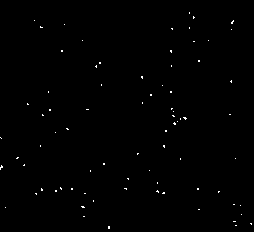
\includegraphics[width=8.5cm]{./images/bacteriasmall_threshold}
        \caption{This represents a segmented and inverted version of the image on the left. White cluster are bacteria.}\label{fig:BBB}
    \end{minipage}
\end{figure*}

 
All the images go through a noise reduction stage which employes a combinations of \textit{gaussian}, \textit{laplacian} and \textit{blurring} filters \cite{Deng:1993}.
Values parameters used in the Contrast Stretching and Threshold filters are dataset dependent and need to be provided upfront. The initial range of colors is affected by optical conditions at the time of the experiment such as lenses, luminosity etc. Once found the best set of parameters for one image, they can be used throughout the whole dataset since all images are taken under the same conditions.

\subsection{Bacteria Tracking}
Binary images are then used to extract the relevant information for each of the segmented bacteria. This is done by interpreting each image as a graph whose nodes are pixels and an arc $(i,j)$ exists if pixels $i$ and $j$ are set and neighbors (according to Moore's relationship). A bacteria correspond then to a connected component that are easily individuated by using an elementary processes which triggers a DFS visit from each set pixel. Once all pixels that make up the cell soma are individuated a unique ID $id_i$ that  identifies the bacterium univoquely, a centroid $c_i$ and a bounding box $s_i$ which describe describes the location, the shape and the area respectively are computed for each bacterium $i$. \texttt{CGAL} \cite{CGAL} is used to create and manipulate any geometrical entities. All the bacteria whose extension is less than $M_e = 2$\textit{px} are ignored and no further considered.

Weight function is a linear combination of the centroides distance and shapes difference 
\[
W(b_i,b_j) = a \sqrt{(c_i.x - c_j.x)^2 + (c_i,y-c_j.y)^2} + b |s_i \cap s_j|
\]
where $s_i$ and $s_j$ are the sets of pixels that within the bacteria bounding box.

 Una volta segmentati  i batteri, per ognuno di essi bisogna calcolarne le informazioni che li identificano univocamente e spazialmente. Abbiamo scelto di utilizzare un poligono (la libreria geometrica usata è CGAL \textbf{(metti riferimento a CGAL importante)}versione random) i cui lati approssimano i contorni del batterio e il relativo centroide ed un ID  univoco che consiste in un intero progressivo. \textbf{Qui ci sta bene un immagine di un batterio segmentato con disegnato il poligono! (Grazie Paola)}
 Tutti batteri segmentati vengono poi filtrati in base a un criterio di conformità che dipende dalle dimensioni del poligono (eliminiamo pixel di dimensione troppo piccola, che magari sono solo rumore residuo o batteri molto fuori fuoco). se l'immagine è interpretata come un grafo allora ogni pixel attivo è un nodo, e  un arco esiste tra due nodi se e solo se le coordinate del nodo differiscono di uno(sono vicini secondo il vicinato di moore). Per ogni componente connessa di questo grafo viene avviata una visita per profondita, ed a tutti i piixel della componente connessa in esame viene asegnato lo stesso ID univoco. (vedi se è il caso di metter una msatrice sintetica di esempio)

Prossima fase è l'individuazione dei batteri a partire dall'immagine binaria. Ogni batterio segmentato viene assegnato un ID univoco all'interno dell'immagine e viene descritto tramite un centroide e un poligono che ne descrive la forma(spiega che libreria viene utilizzata CGAL, in che versione)
Quanti batteri mediamente ci sono? 


spiega che i batteri si muovo in unoi spazio 3d e che il fuoco del microscopio è molto stretto (servono dati sul fuoco del microscopio) e che una volta che i batteri nuotano in direzione Y scompaiono dalle immagini. 
Se una particella(cosi vengono chiamte nella descrizione dell'algoritmo al capitolo precedente) è "scompars" per un certo numero di frames, fino a quando la consideriamo candidabile per un eventuale match?

Durante la validazione dei risultati è importante dire che i primi test sono stati effettuati utilizzando immagini  sintetiche di cluster non omogenei di pixel colorati su sfondo nero e fatti muovere secondo un certo movimento  (inventatene uno figo, circolare, pseudorandom blabla). 
Mostra qualche risultato, ad esempio la velocità di movimento matcha. 
\subsection{Tracking}
In questa sezione bisogna specificare tutte le "funzioni" dell'algoritmo di tracking che sono state overriddate e "tunate" per questo specifico problema. Per esempio che funzione di distanza è stata utilizzata (mi pare che utilizziamo la similiarità dei poligono, e la distanza in una media pesata, ricorda di mettere i valori dei parametri che empiricamente hanno mostrato i migliori risultati)?
Cosa sputa fuori in output?  

\section{Conclusion}
scopo: inferire modelli matematici che descrivono 

toglie i tumble e checcka speed del run
come vengono checkati i tumble?
18micrometri al secondo risultato
tubling di 0.2 -> running 1-0.2 =0.8 sec
in bio il dato è cvariabile perche va da 15 a 30 (dipende dalla ref) ma ha senso dal punto di vista bio
va giustificato con delle referenza con i Bsaptisolis

2) track analizzate msd analyzer

variazione nel tempo del msd => legata al coeff di diffusione
 => legato a due cose : velocità e il tempo di tumble
 23 con questo metodo. biologicamente sono buoni (18 e 23) sono compatibili con veliocità di sti batteri
 
quindi se con due modi diversi trovi risultati builogicamente buoni => tracking funge




Come è stato validato il modello? (dovrebbe scriverlo alice)

    \begin{figure}
      \begin{center}
        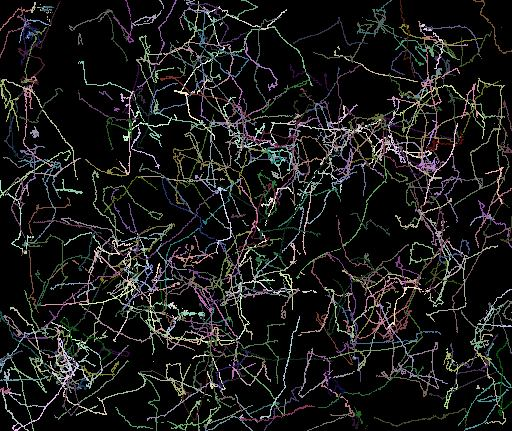
\includegraphics[scale=0.5]{./images/result.png}
        \caption{Trajectories}
        \label{fig:}
      \end{center}
    \end{figure}





% if have a single appendix:
%\appendix[Proof of the Zonklar Equations]
% or
%\appendix  % for no appendix heading
% do not use \section anymore after \appendix, only \section*
% is possibly needed

% use appendices with more than one appendix
% then use \section to start each appendix
% you must declare a \section before using any
% \subsection or using \label (\appendices by itself
% starts a section numbered zero.)
%


\appendices
\section{Images Filters}
\subsection{contrast stretch}

% use section* for acknowledgement
\section*{Acknowledgment}


The authors would like to thank...


% Can use something like this to put references on a page
% by themselves when using endfloat and the captionsoff option.
\ifCLASSOPTIONcaptionsoff
  \newpage
\fi



% trigger a \newpage just before the given reference
% number - used to balance the columns on the last page
% adjust value as needed - may need to be readjusted if
% the document is modified later
%\IEEEtriggeratref{8}
% The "triggered" command can be changed if desired:
 ì%\IEEEtriggercmd{\enlargethispage{-5in}}

% references section

% can use a bibliography generated by BibTeX as a .bbl file
% BibTeX documentation can be easily obtained at:
% http://www.ctan.org/tex-archive/biblio/bibtex/contrib/doc/
% The IEEEtran BibTeX style support page is at:
% http://www.michaelshell.org/tex/ieeetran/bibtex/
%\bibliographystyle{IEEEtran}
% argument is your BibTeX string definitions and bibliography database(s)
%\bibliography{IEEEabrv,../bib/paper}
%
% <OR> manually copy in the resultant .bbl file
% set second argument of \begin to the number of references
% (used to reserve space for the reference number labels box)
\begin{thebibliography}{1}

\bibitem{Cho:1989}
S. Cho, R. Haralick, and S. Yi, “Improvement of Kittler and Illingworth’s minimum error thresholding,” Pattern Recognit., vol. 22, no. 5, pp. 609– 617, 1989.
\bibitem{Shapiro:2002}
Shapiro, Linda G, Stockman, George C. (2002). "Computer Vision". Prentice Hall. ISBN 0-13-030796-3

\bibitem{Deng:1993} 
G. Deng and L. W. Cahill, An adaptive Gaussian filter for noise reduction and edge detection, Nuclear Science Symposium and Medical Imaging Conference, 1993. 1615-1619 vol.3, 10.1109/NSSMIC.1993.373563

\bibitem{CGAL}
CGAL, Computational Geometry Algorithms Library, http://www.cgal.org
\end{thebibliography}

% biography section
% 
% If you have an EPS/PDF photo (graphicx package needed) extra braces are
% needed around the contents of the optional argument to biography to prevent
% the LaTeX parser from getting confused when it sees the complicated
% \includegraphics command within an optional argument. (You could create
% your own custom macro containing the \includegraphics command to make things
% simpler here.)
%\begin{biography}[{\includegraphics[width=1in,height=1.25in,clip,keepaspectratio]{mshell}}]{Michael Shell}
% or if you just want to reserve a space for a photo:

\begin{IEEEbiography}[{\includegraphics[width=1in,height=1.25in,clip,keepaspectratio]{picture}}]{John Doe}
\blindtext
\end{IEEEbiography}

% You can push biographies down or up by placing
% a \vfill before or after them. The appropriate
% use of \vfill depends on what kind of text is
% on the last page and whether or not the columns
% are being equalized.

%\vfill

% Can be used to pull up biographies so that the bottom of the last one
% is flush with the other column.
%\enlargethispage{-5in}


\section{Multi GPU-MPI not part of the paper}
Sharing data via GPUs is done via
\begin{itemize}
	\item Explicit copy via host
	\item Zero-copy shared host array
	\item Per device arrays peer-to-peer echange
	\item Peer-to-peer memory access
\end{itemize}
A single host can have multiple cuda context (i.e. works with multiple GPU) and can switch between them using \texttt{cudaSetDevice}.
Multiple hosts can establish context with the \textbf{same} GPU (the drivers take care of the resource sharing among the hosts!

A simple and naive approach is to run multiple independent kernels on different devices.

Cuda offers the possibility to control multiple GPUs from the same thread withouth need of CPU multithreading (single CPU host can control a number of devices).
With \textbf{cuda streams} memcopies can be performed in parallel (up to 2 tough)
Memo copies can also be performed without using the host at all. It's called peer-to-peer memory copy and is performed among GPUs attached to the \textbf{same} PCIe switch using \texttt{cudaMemcpyPeerAsync} API. 
Disjoint set of GPU can communicate simulaneously. (Imagine 4 GPU in the same machine. GPUs (1,3) communicate using peer-to-peer mamory transfer and GPUs (0,2) can do the same thing at the same exact time )
\end{document}


